\begin{transitionframe}
	\begin{center}
		{ \Huge \textcolor{black}{Técnicas de Escalonamento}}
	\end{center}
\end{transitionframe}

\begin{frame}{Min-Max}
\begin{center}
	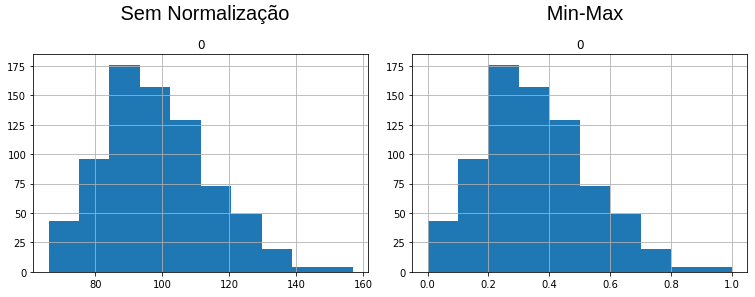
\includegraphics[width=.9\textwidth,height=.7\textheight]{./fig/sem_min_max.png}
\end{center}
\end{frame}

\begin{frame}{Standard}
\begin{center}
	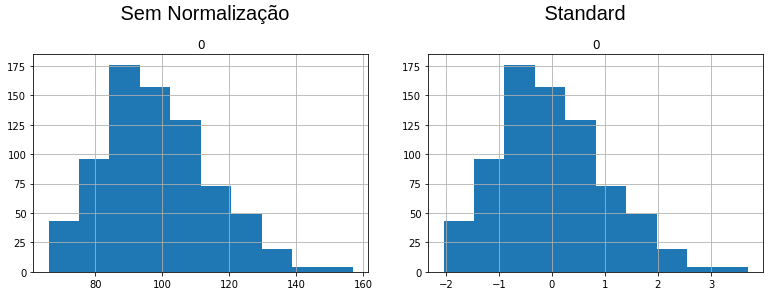
\includegraphics[width=.9\textwidth,height=.7\textheight]{./fig/sem_std.png}
\end{center}
\end{frame}

\begin{frame}{Max Absolute}
\begin{center}
	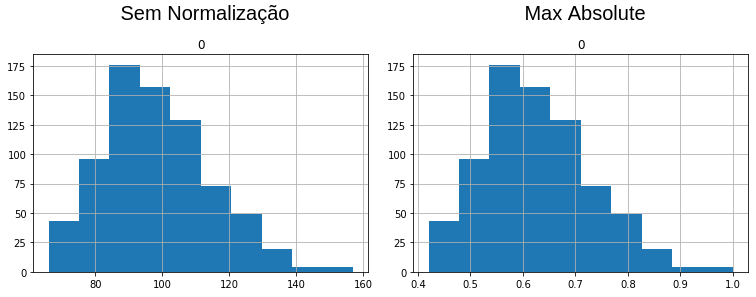
\includegraphics[width=.9\textwidth,height=.7\textheight]{./fig/sem_max_abs.png}
\end{center}
\end{frame}

\begin{frame}{Robust}
\begin{center}
	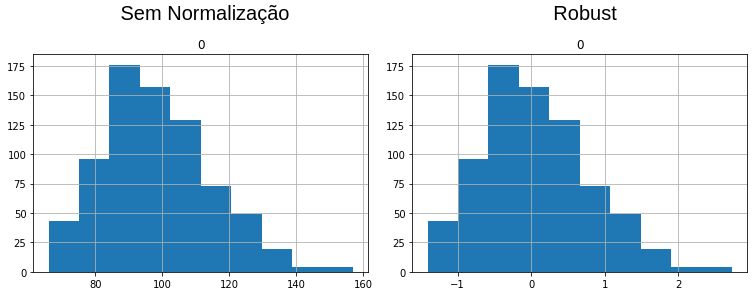
\includegraphics[width=.9\textwidth,height=.7\textheight]{./fig/sem_rbt.png}
\end{center}
\end{frame}

\begin{frame}{Técnica de Escalonamento para o descritor LBP}
\begin{center}
	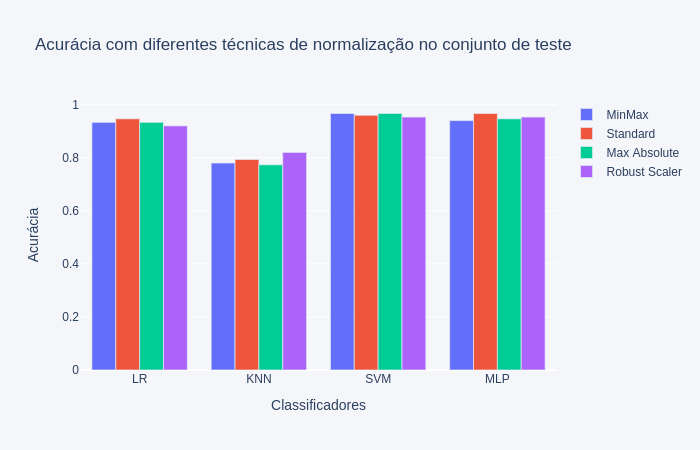
\includegraphics[width=.8\textwidth,height=.7\textheight]{./fig/bar_norm_all_lbp.png}
\end{center}
Fonte: \emph{\textcolor{blue}{\href{https://colab.research.google.com/drive/15Ozutw22u9wfAXisgqfhmA33P3s0fbWp?usp=sharing}{Colab}}}
e
\emph{\textcolor{blue}{\href{https://github.com/guimpo/hand_on_again_ai_master/}{GitHub}}}
\end{frame}

\begin{frame}{Técnica de Escalonamento para o descritor Gabor}
\begin{center}
	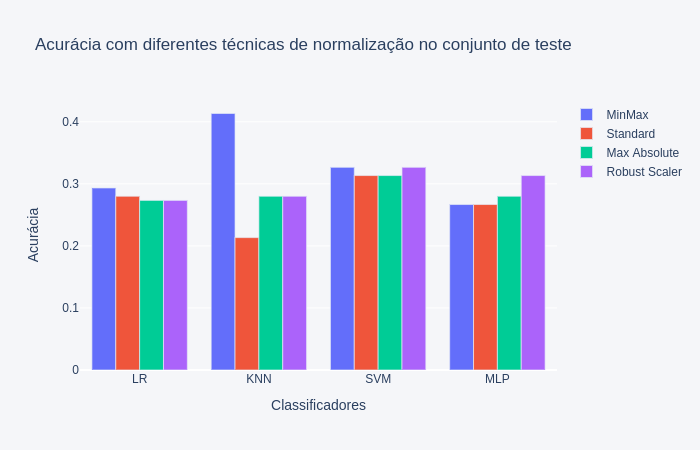
\includegraphics[width=.8\textwidth,height=.7\textheight]{./fig/bar_norm_all_gabor.png}
\end{center}
Fonte: \emph{\textcolor{blue}{\href{https://colab.research.google.com/drive/15Ozutw22u9wfAXisgqfhmA33P3s0fbWp?usp=sharing}{Colab}}}
e
\emph{\textcolor{blue}{\href{https://github.com/guimpo/hand_on_again_ai_master/}{GitHub}}}
\end{frame}